\documentclass[12pt]{article}
\usepackage[pdftex]{graphicx}
\usepackage{fullpage}
\usepackage[T1]{fontenc}
\begin{document}
\begin{center}
\textbf{filename: \expandafter\detokenize\expandafter{\myvar}}
\textbf{Window Size: \expandafter\detokenize\expandafter{\window}}


\textbf{Plot with different regressions in the Beta Band (12-30) }
\end{center}

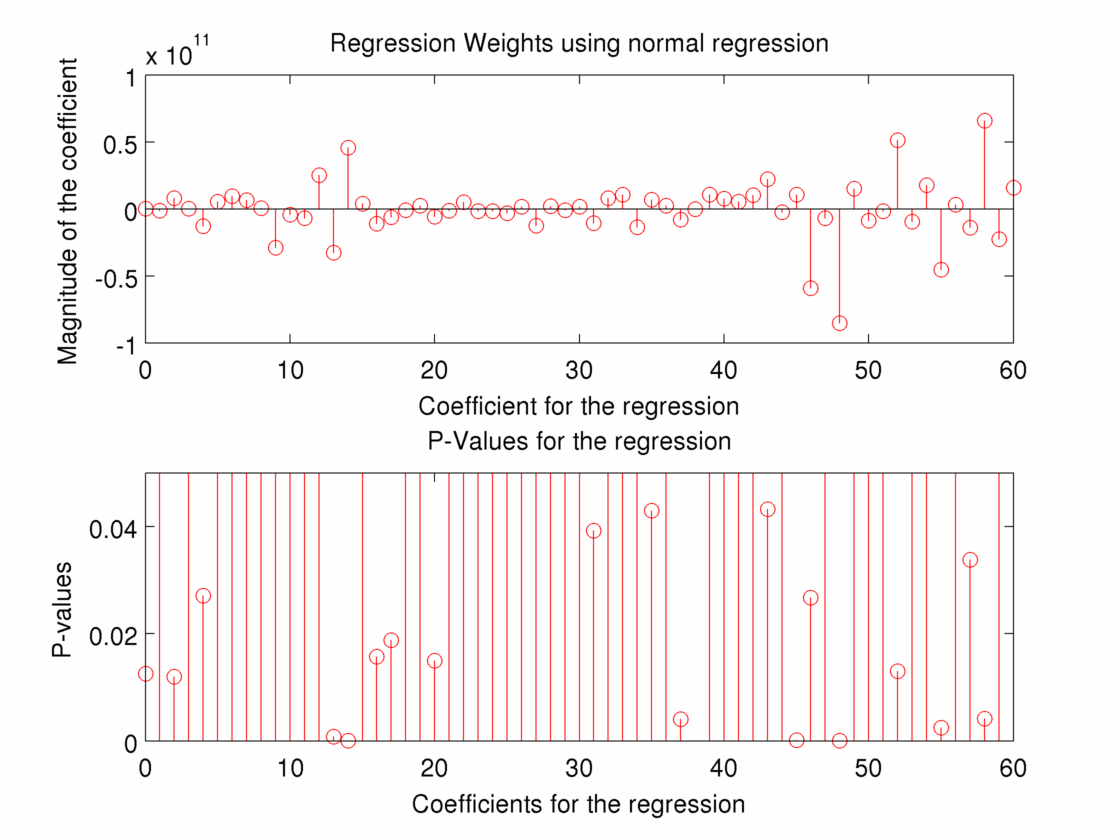
\includegraphics[scale=0.2]{regression_weights_p_value.png}
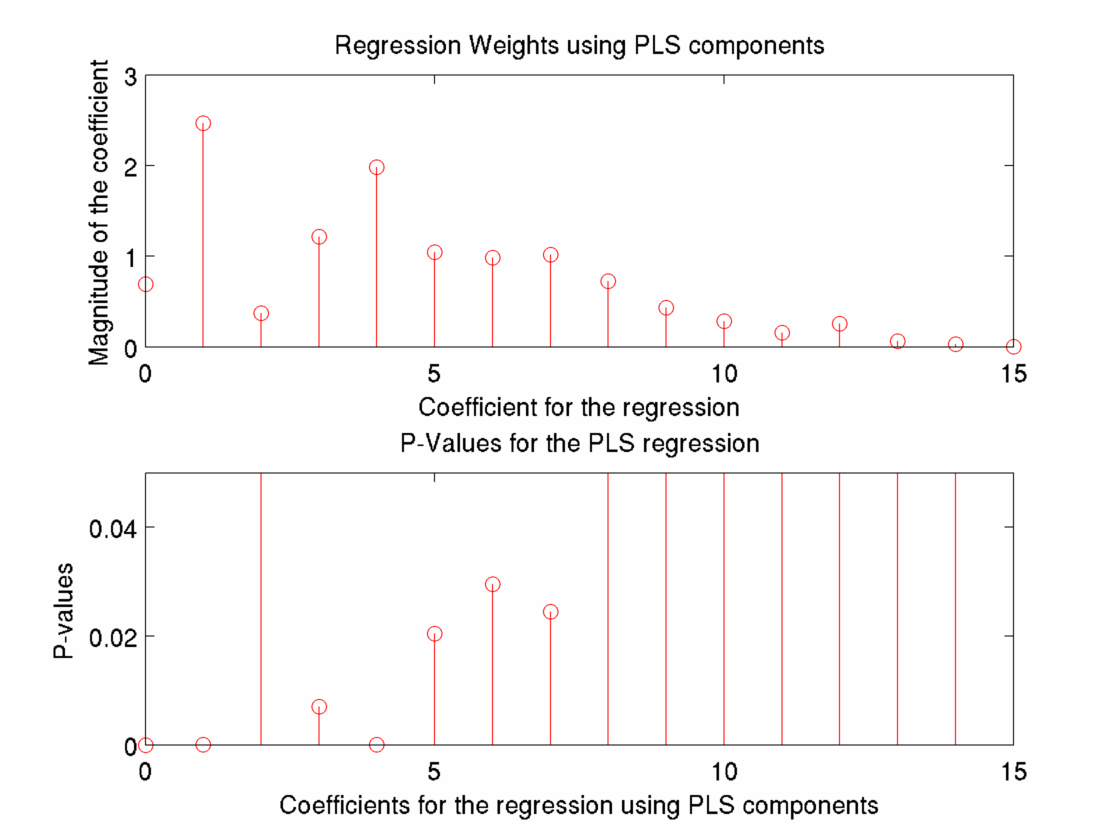
\includegraphics[scale=0.2]{glmfit_regression_pls.png}

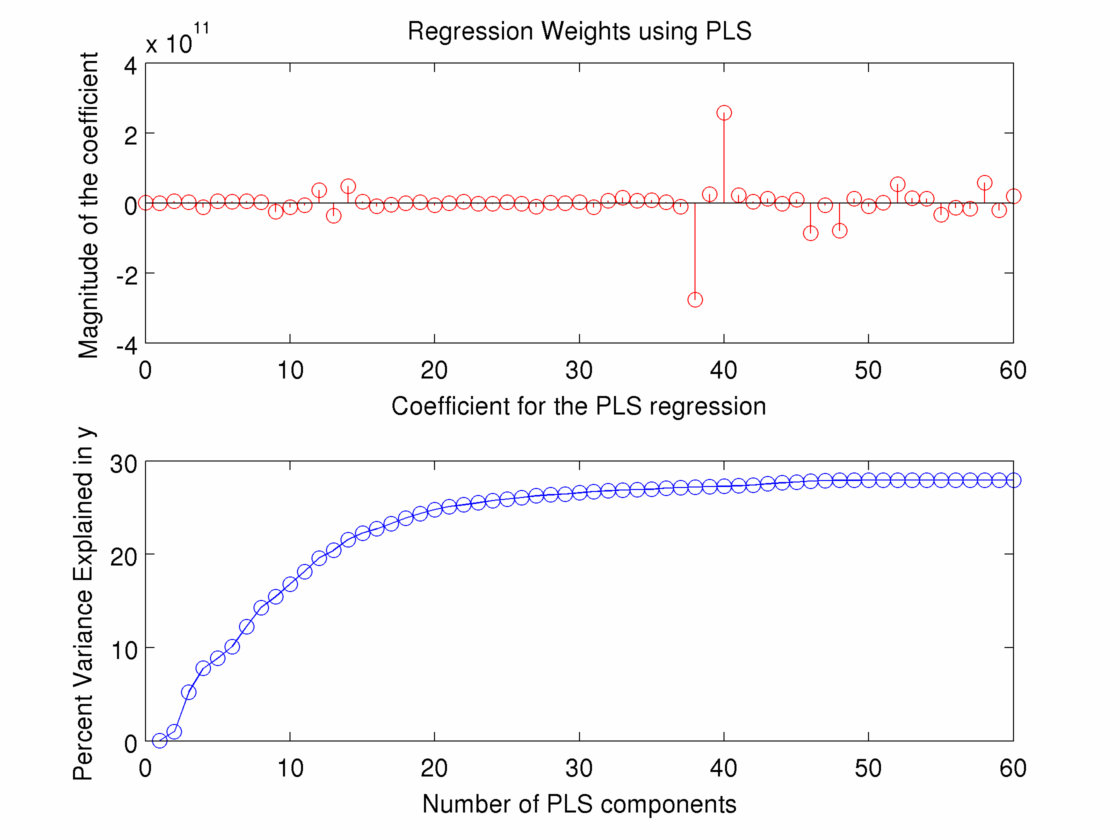
\includegraphics[scale=0.2]{pls_regression_weights_pctvar.png}
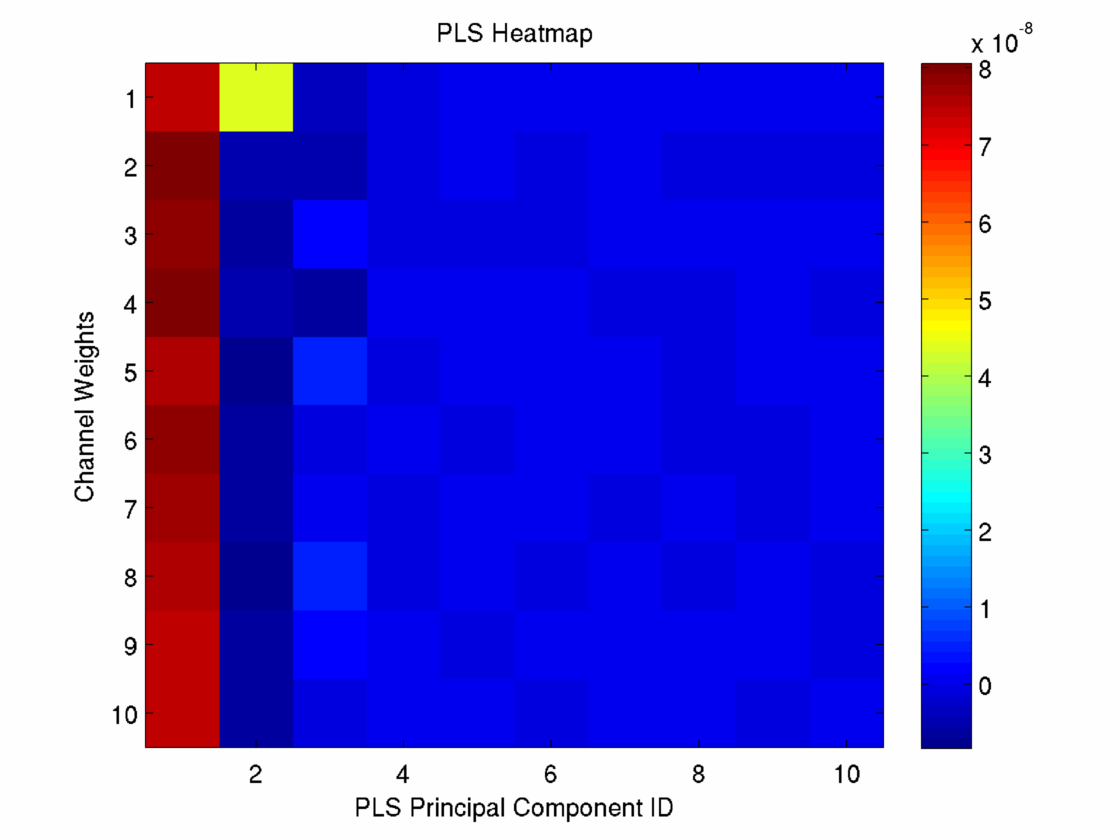
\includegraphics[scale=0.2]{PLS_heatmap.png}


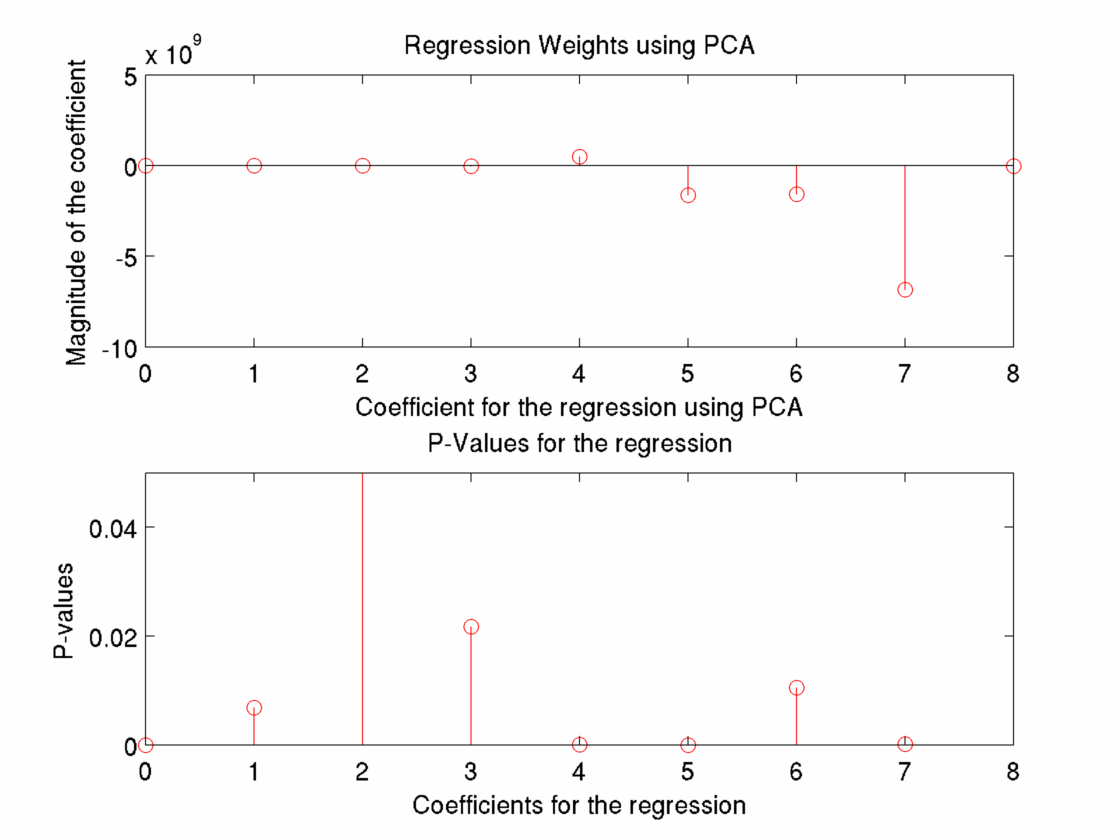
\includegraphics[scale=0.2]{PCA_regression_weights_p_value.png}
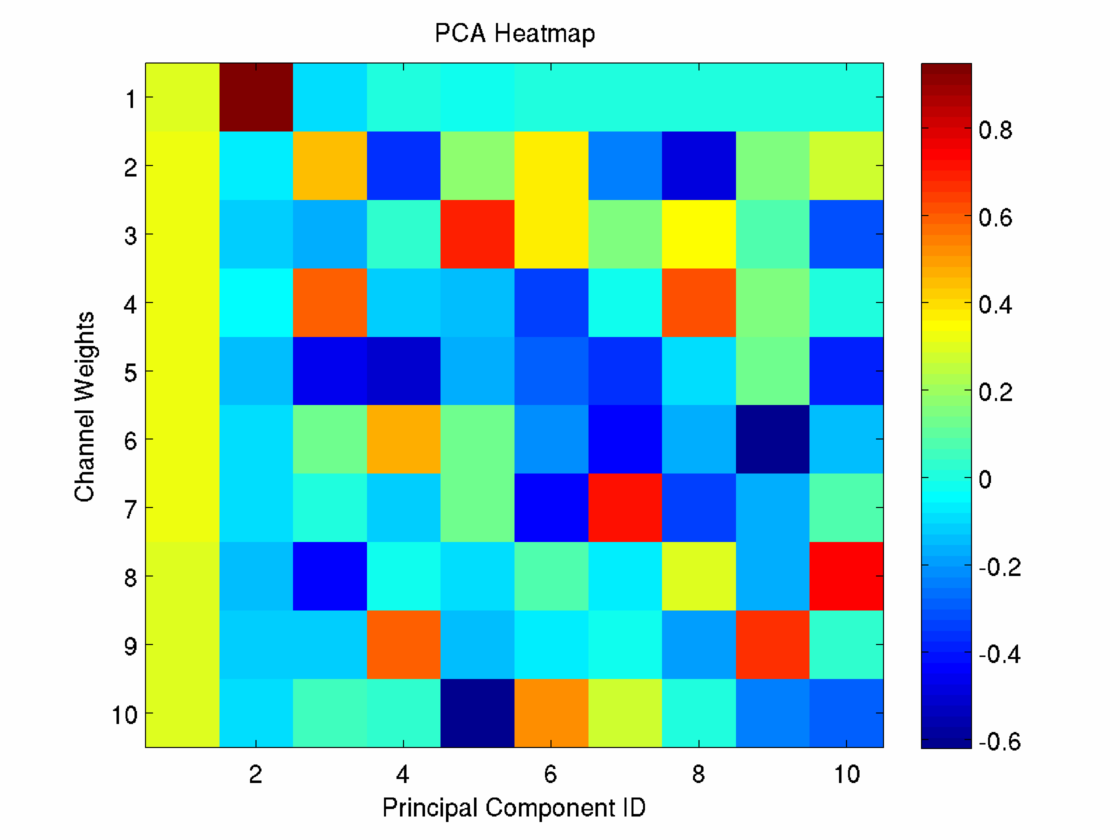
\includegraphics[scale=0.2]{PCA_heatmap.png}

\newpage
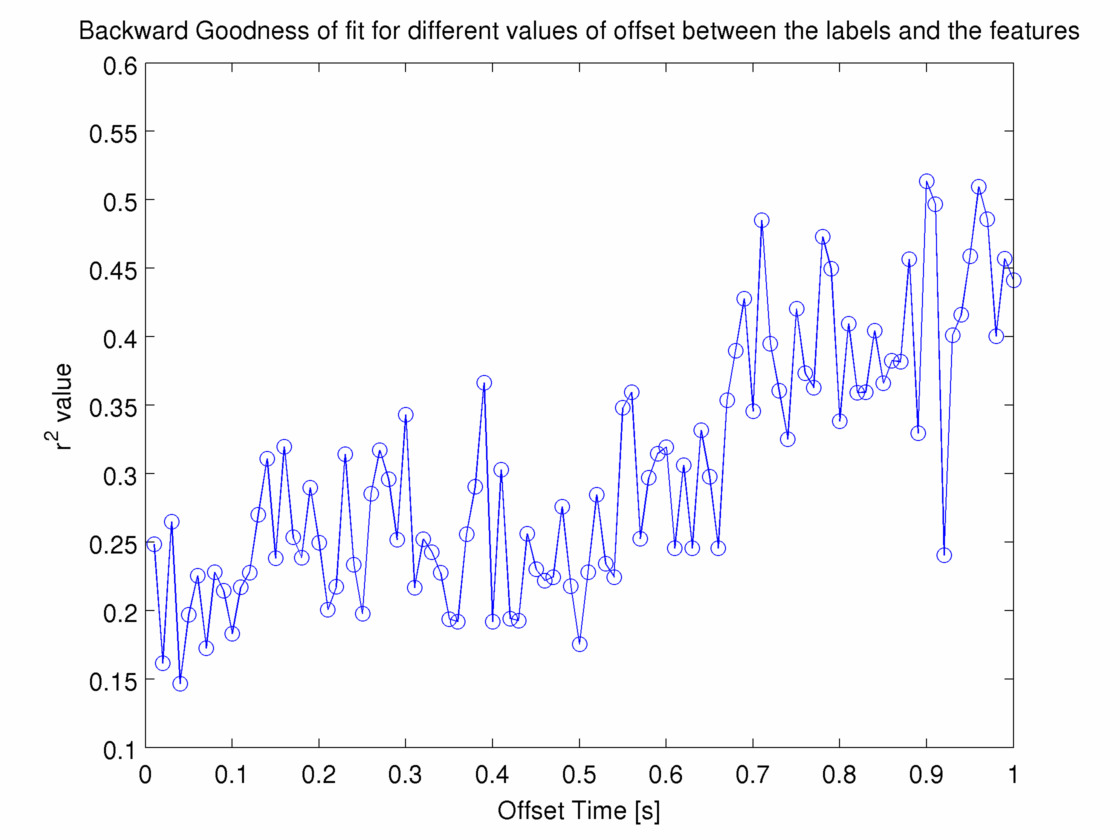
\includegraphics[scale=0.2]{regression_r_value_forward.png}
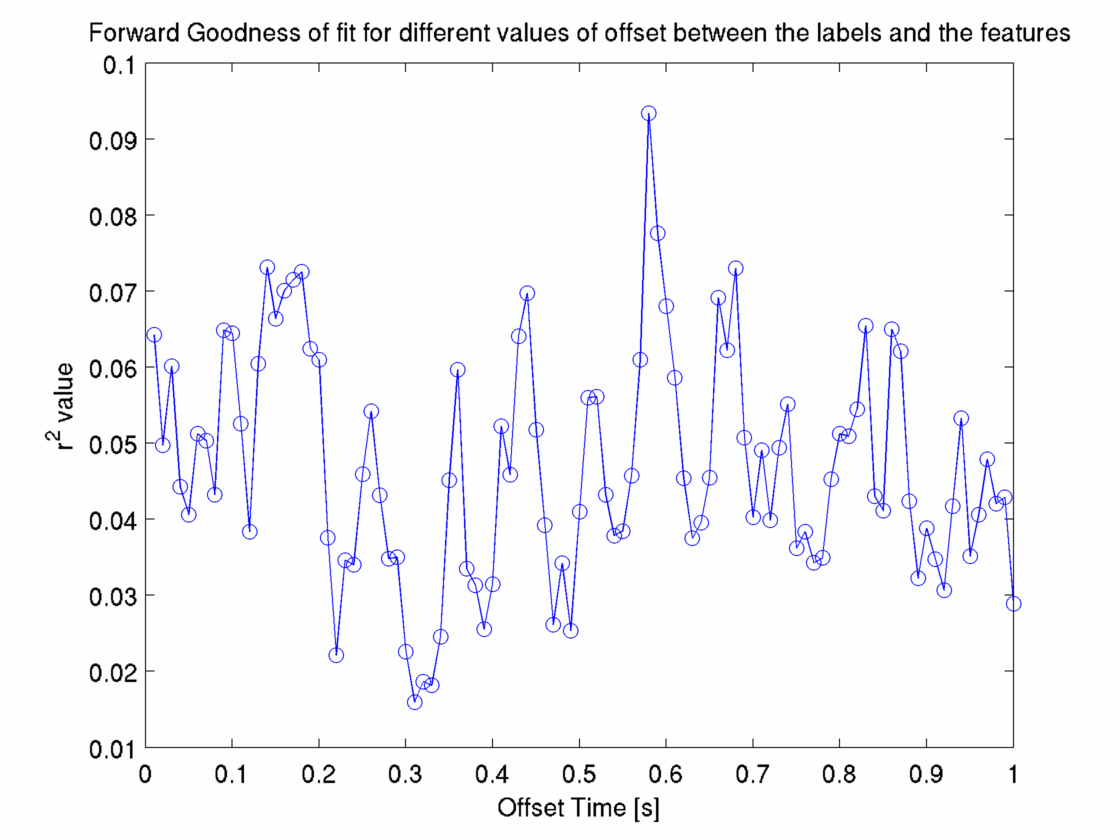
\includegraphics[scale=0.2]{regression_r_value_backward.png}

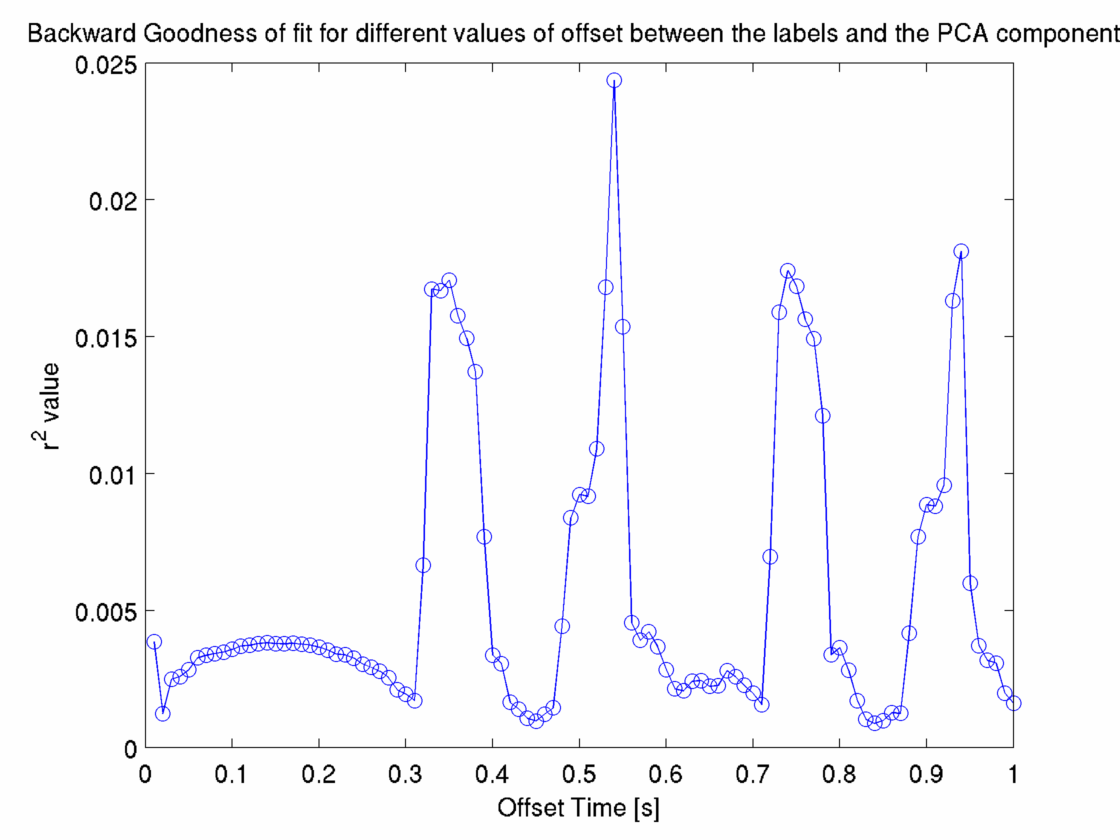
\includegraphics[scale=0.2]{pca_regression_r_value_forward.png}
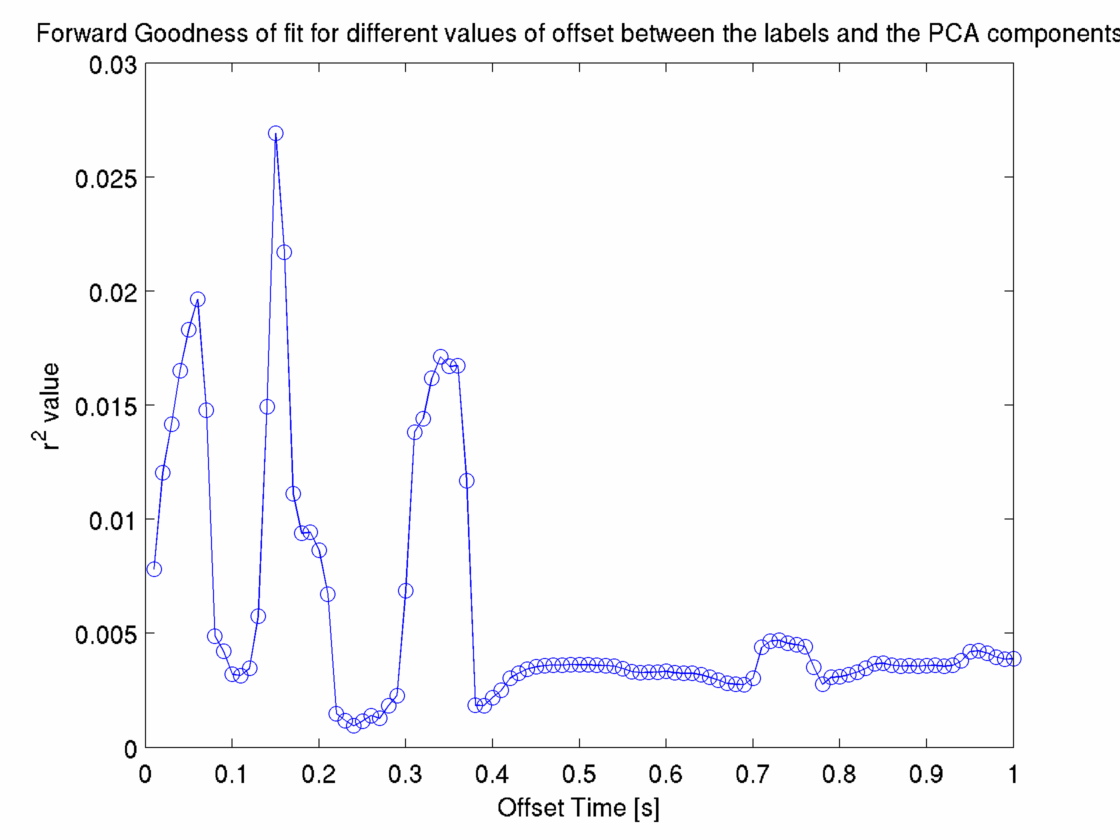
\includegraphics[scale=0.2]{pca_regression_r_value_backward.png}

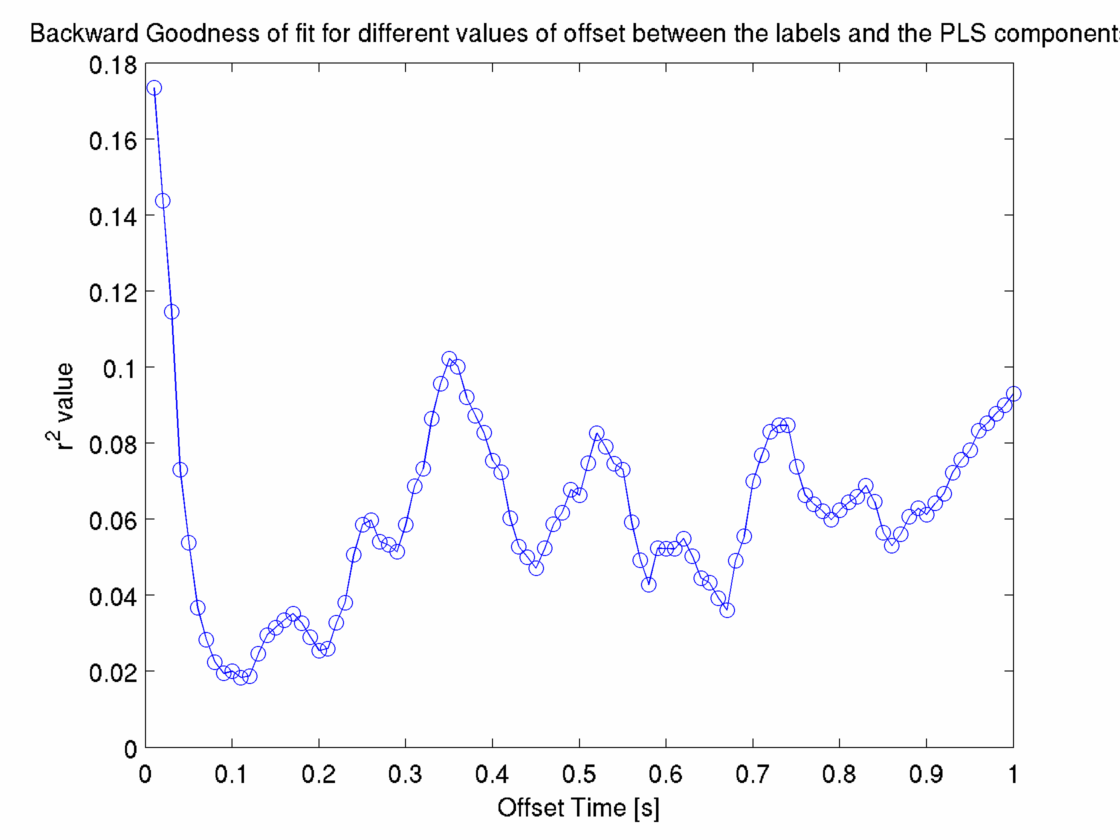
\includegraphics[scale=0.2]{pls_regression_r_value_forward.png}
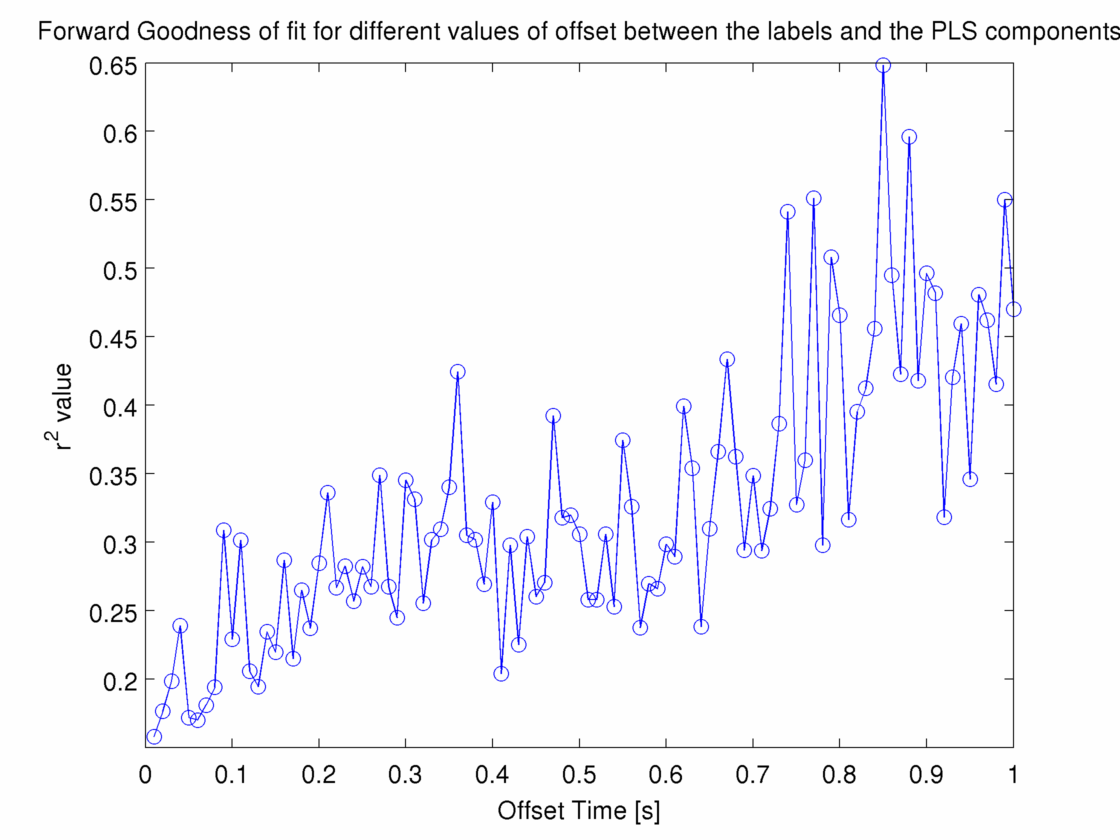
\includegraphics[scale=0.2]{pls_regression_r_value_backward.png}

\newpage
\begin{center}
\textbf{filename: \expandafter\detokenize\expandafter{\myvar}}
\textbf{Window Size: \expandafter\detokenize\expandafter{\window}}


\textbf{Plot with different regressions for all the bands }
\end{center}
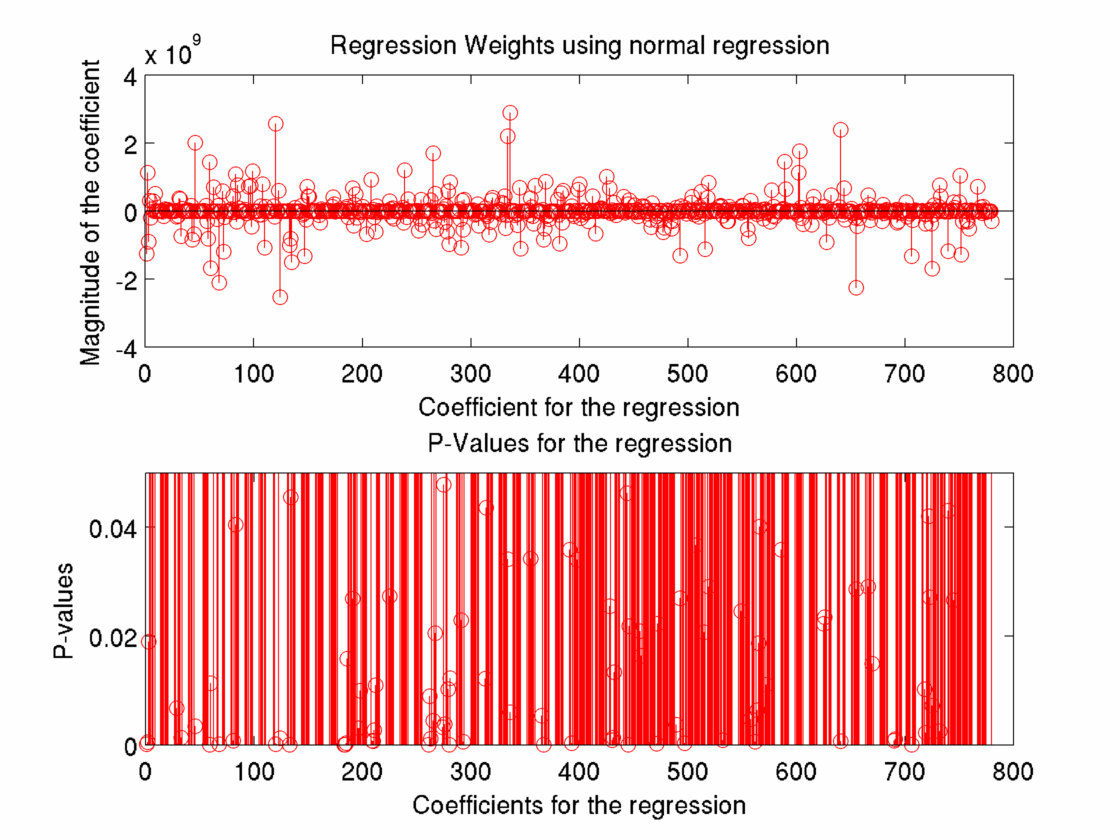
\includegraphics[scale=0.2]{full_regression_weights_p_value.png}
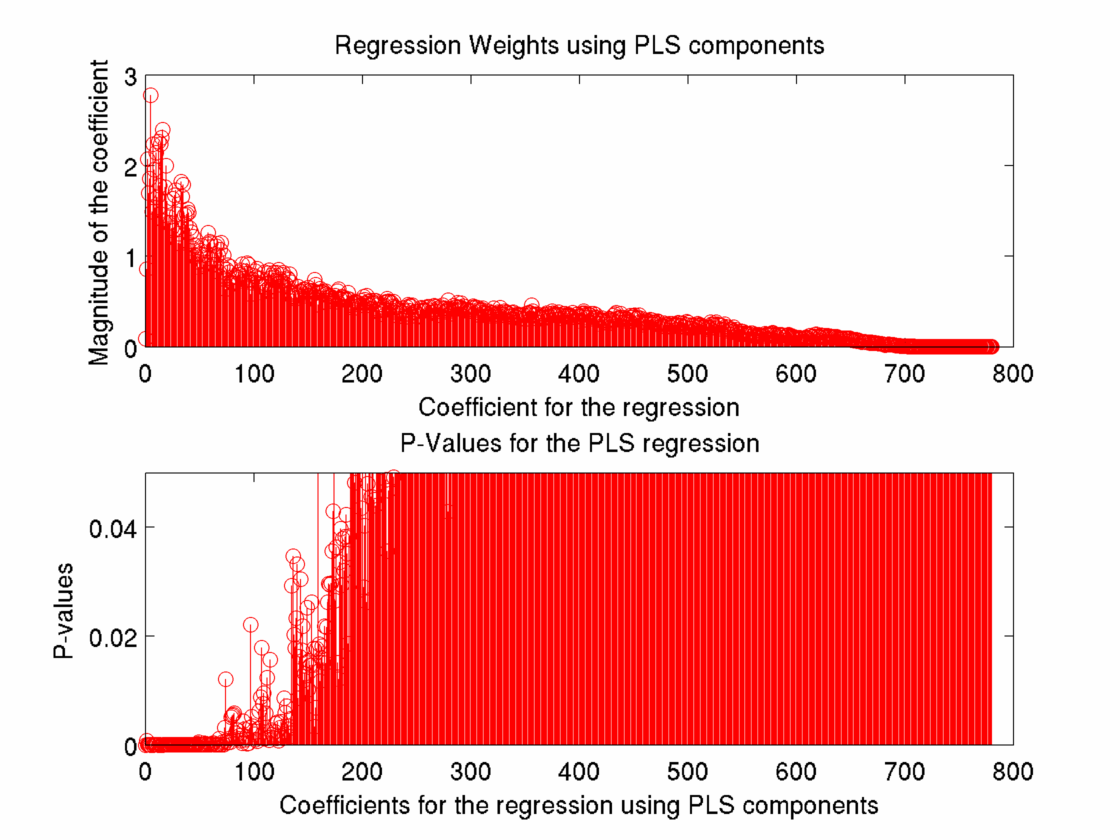
\includegraphics[scale=0.2]{full_glmfit_regression_pls.png}

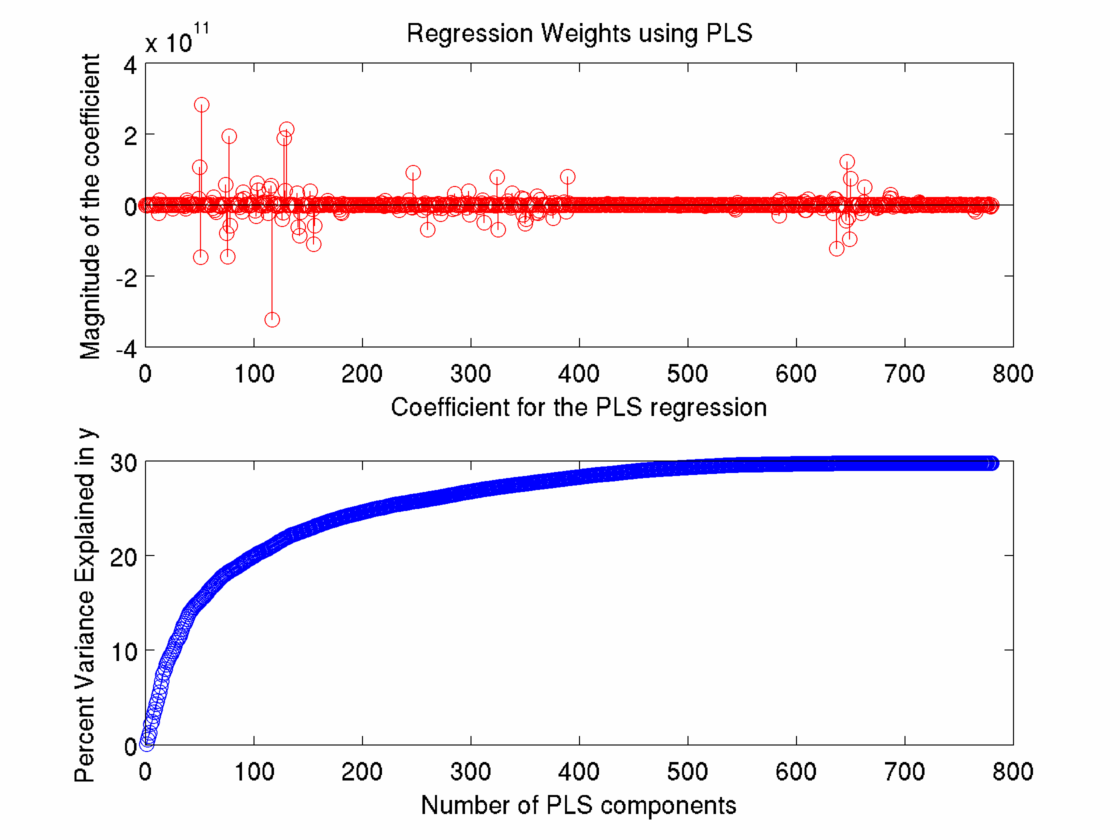
\includegraphics[scale=0.2]{full_pls_regression_weights_pctvar.png}
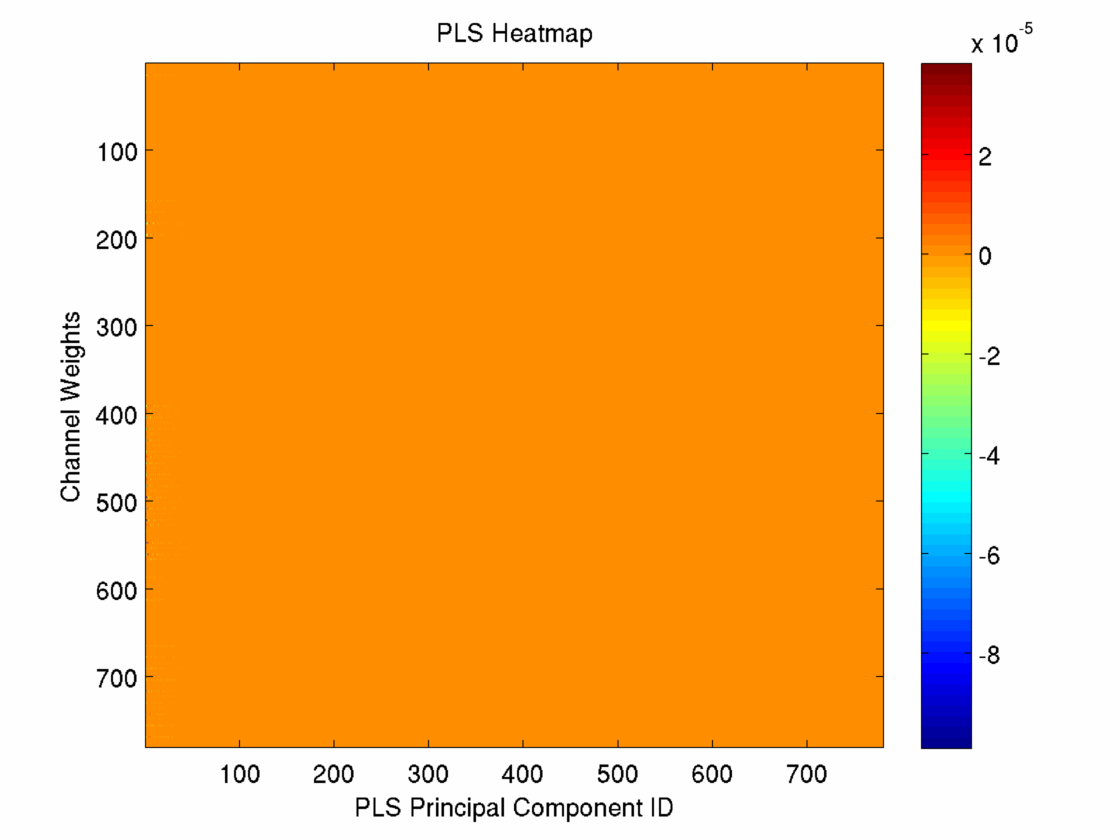
\includegraphics[scale=0.2]{full_PLS_heatmap.png}


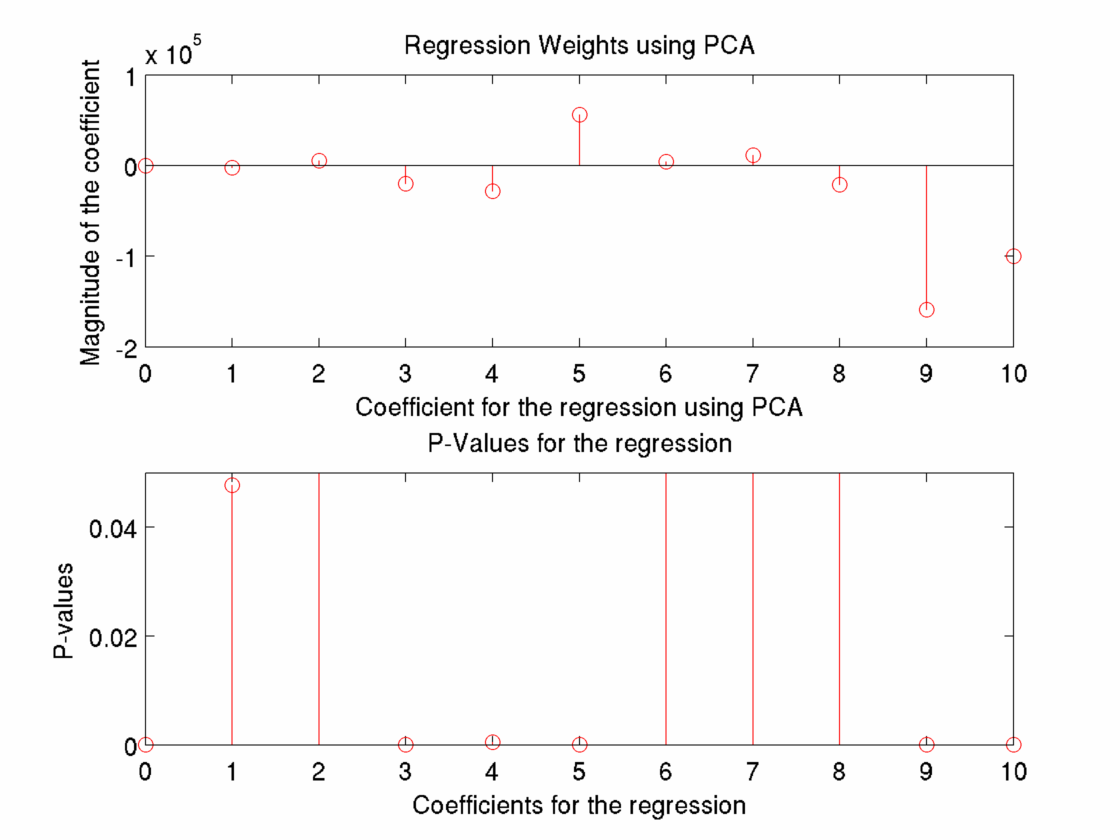
\includegraphics[scale=0.2]{full_PCA_regression_weights_p_value.png}
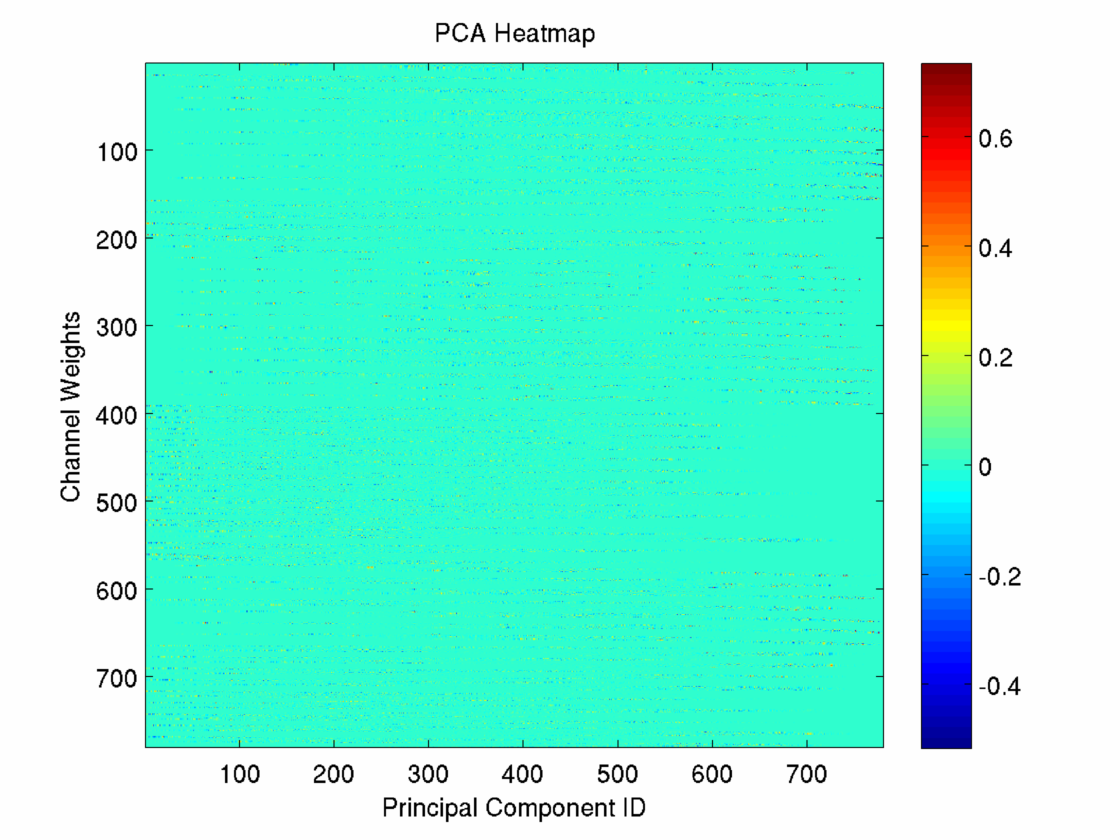
\includegraphics[scale=0.2]{full_PCA_heatmap.png}
\end{document}